\documentclass[aspectratio=169,11pt]{beamer}

\usepackage[utf8]{inputenc}
\usepackage[T1]{fontenc}
\usepackage[brazilian]{babel}
\usepackage{graphicx}
\usepackage{booktabs}
\usepackage{amsmath}

\usetheme{Madrid}
\usecolortheme{default}

\definecolor{UfpiNavy}{RGB}{30,58,138}
\definecolor{OptGreen}{RGB}{21,128,61}
\definecolor{WarnRed}{RGB}{185,28,28}

\setbeamercolor{structure}{fg=UfpiNavy}
\setbeamercolor{palette primary}{bg=UfpiNavy,fg=white}
\setbeamercolor{palette secondary}{bg=UfpiNavy!85!black,fg=white}
\setbeamercolor{palette tertiary}{bg=UfpiNavy!70!black,fg=white}
\setbeamercolor{frametitle}{bg=UfpiNavy,fg=white}
\setbeamercolor{block title}{bg=UfpiNavy,fg=white}
\setbeamercolor{block title example}{bg=OptGreen,fg=white}
\setbeamercolor{block title alerted}{bg=WarnRed,fg=white}
\setbeamertemplate{navigation symbols}{}

\graphicspath{{../paper/figures/}}

\title[Indexação e Otimização no SQL Server 2022]{Análise Experimental de Indexação, Planos de Execução e Otimização de Consultas no SQL Server 2022}
\subtitle{Trabalho Final -- Banco de Dados II (2026.2) | Prof. Dennis Sávio}
\author[Hermeson A. et al.]{Hermeson A., João Marcos R., Lizzandro W.,\texorpdfstring{\\}{ }Marcos W., Raildom R.}
\institute[UFPI/CSHNB]{Bacharelado em Sistemas de Informação\\Universidade Federal do Piauí (UFPI) -- CSHNB -- Picos -- PI}
\date{Novembro de 2026}

\begin{document}

\begin{frame}
  \titlepage
\end{frame}

\begin{frame}{1. Motivação e Problema de Pesquisa}
  \begin{columns}[T]
    \begin{column}{0.48\textwidth}
      \begin{block}{Gargalos em Escala (Milhões de Linhas)}
        \begin{itemize}
          \item \textbf{Varreduras integrais (\textit{Scan}):} custo $O(N)$ satura o \textit{buffer pool} e o barramento de E/S.
          \item \textbf{\textit{Key Lookups} aleatórios:} buscas repetidas na tabela base anulam ganhos parciais.
          \item \textbf{SQL não-\textit{sargable}:} funções sobre colunas (\texttt{YEAR}) e curingas iniciais (\texttt{'\%...'}) bloqueiam índices.
        \end{itemize}
      \end{block}
    \end{column}
    \begin{column}{0.48\textwidth}
      \begin{alertblock}{O Mito do ``Índice Gratuito''}
        \begin{itemize}
          \item Índices B+ aceleram leituras, mas exigem escrita síncrona (\textit{write amplification}).
          \item Menor E/S nem sempre equivale a menor latência de CPU (\textit{Batch Mode} vs. \textit{Row Mode}).
        \end{itemize}
      \end{alertblock}
      \begin{exampleblock}{Objetivo}
        Quantificar ganhos reais e \textit{trade-offs} no \textbf{SQL Server 2022} com rigor estatístico ($N=30$ \textit{Warm}, $N=10$ \textit{Cold}).
      \end{exampleblock}
    \end{column}
  \end{columns}
\end{frame}

\begin{frame}{2. Referencial Teórico: Árvores B+ e Estratégias de Índice}
  \begin{columns}[T]
    \begin{column}{0.52\textwidth}
      \begin{block}{Estrutura em Páginas de 8 KB (Comer, 1979)}
        \begin{itemize}
          \item \textbf{Clusterizado:} folhas armazenam as linhas completas (1 por tabela).
          \item \textbf{Não-clusterizado:} folhas guardam chave + chave clusterizada como localizador ($O(\log_m N)$).
          \item \textbf{Índice de Cobertura (\texttt{INCLUDE}):} replica atributos não-chave nas folhas para eliminar \textit{Key Lookups}.
        \end{itemize}
      \end{block}
    \end{column}
    \begin{column}{0.44\textwidth}
      \begin{block}{Especializações Avaliadas}
        \begin{itemize}
          \item \textbf{Composto \texttt{(Status, DataPedido)}:} igualdade à esquerda, faixa à direita.
          \item \textbf{Filtrado (\texttt{WHERE Desconto >= 10.00}):} indexa apenas $\sim$20\% da tabela, reduzindo altura e escrita.
          \item \textbf{Custo DML:} cada \texttt{INSERT} atualiza todas as B+ Trees da tabela.
        \end{itemize}
      \end{block}
    \end{column}
  \end{columns}
\end{frame}

\begin{frame}{3. Otimizador Baseado em Custos e Modos de Execução}
  \begin{itemize}
    \item \textbf{Reescrita e Sargabilidade (System R / Cascades):}
      \begin{itemize}
        \item \texttt{YEAR(DataPedido) = 2025} $\rightarrow$ intervalo semiaberto \texttt{[2025-01-01, 2026-01-01)}.
        \item \texttt{LIKE N'\%Notebook\%'} $\rightarrow$ busca por prefixo \texttt{LIKE N'Notebook\%'} (quando válido no domínio).
        \item Subconsulta agregada correlacionada $\rightarrow$ \texttt{NOT EXISTS} (\textit{Left Anti Semi Join}).
      \end{itemize}
    \item \textbf{Operadores Físicos de Junção:} \textit{Nested Loops} (poucas linhas + índice), \textit{Merge Join} (entradas ordenadas) e \textit{Hash Match} (volumes grandes não ordenados).
    \item \textbf{\textit{Batch Mode on Rowstore} (SQL Server 2022):} processa vetores de tuplas em lote (\textit{Hash Match}), superando \textit{Row Mode} (\textit{Stream Aggregate}) intensivo em CPU.
  \end{itemize}
\end{frame}

\begin{frame}{4. Metodologia: Ambiente Reprodutível e Bases Gêmeas}
  \begin{columns}[T]
    \begin{column}{0.49\textwidth}
      \begin{block}{Infraestrutura e Dados (6.250.000 linhas)}
        \begin{itemize}
          \item \textbf{Motor:} SQL Server 2022 RTM-CU28 (\textit{Developer}) em Docker (Ubuntu 22.04, 4 GB RAM).
          \item \textbf{Host:} Windows 11, Core i5-1235U, 15,71 GB RAM, SSD.
          \item \textbf{Esquema B2C (\texttt{seed=42}, 400 MB alocados):} \texttt{Clientes} (200k), \texttt{Produtos} (50k), \texttt{Pedidos} (1,5M), \texttt{ItensPedido} (4,5M).
          \item \textbf{Clonagem:} \texttt{BACKUP}/\texttt{RESTORE} mantendo dados e estatísticas iniciais idênticos.
        \end{itemize}
      \end{block}
    \end{column}
    \begin{column}{0.47\textwidth}
      \begin{block}{Baseline vs. Otimizado}
        \begin{itemize}
          \item \texttt{Ecommerce\_Baseline}: 4 PKs clusterizadas, \textbf{0 índices secundários}.
          \item \texttt{Ecommerce\_Otimizado}: \textbf{9 índices secundários} (amostragem estatística de 100\%).
          \item \textbf{Isolamento:} \texttt{OPTION (MAXDOP 1)} e literais tipados sem conversão implícita.
          \item \textbf{Escrita ($W_1$):} encapsulada em \texttt{BEGIN TRAN ... ROLLBACK}.
        \end{itemize}
      \end{block}
    \end{column}
  \end{columns}
\end{frame}

\begin{frame}{5. Carga de Trabalho ($Q_1$--$Q_{10}$, $W_1$) e Protocolo Estatístico}
  \begin{columns}[T]
    \begin{column}{0.58\textwidth}
      \scriptsize
      \setlength{\tabcolsep}{3pt}
      \begin{tabular}{@{}lll@{}}
        \toprule
        \textbf{Cód.} & \textbf{Alvo} & \textbf{Técnica} \\
        \midrule
        $Q_1$ & E-mail pontual (1 linha) & \textit{Seek + Lookup} simples \\
        $Q_2, Q_9$ & Datas / \texttt{YEAR()} & Cobertura + semiaberto \\
        $Q_3$ & \texttt{Status} + data & Composto \texttt{(Status, Data)} \\
        $Q_4$ & Cliente (422 linhas) & \textit{Covering} sem \textit{Lookup} \\
        $Q_5, Q_{10}$ & Junções / \texttt{NOT EXISTS} & \textit{Merge} + \textit{Anti Semi Join} \\
        $Q_6$ & \texttt{TOP 50} recentes & \texttt{BACKWARD} sem \textit{Sort} \\
        $Q_7$ & Soma por \texttt{Status} & \textit{Hash [Batch]} vs. \textit{Stream [Row]} \\
        $Q_8$ & Catálogo (\texttt{LIKE}) & Prefixo sargable vs. \texttt{\%...\%} \\
        $W_1$ & \texttt{INSERT} 10k itens & Escrita em 3 índices sec. \\
        \bottomrule
      \end{tabular}
    \end{column}
    \begin{column}{0.39\textwidth}
      \begin{block}{Coleta e Testes (880 execuções)}
        \footnotesize
        \begin{itemize}
          \item \textbf{Warm Cache:} 2 aquecimentos + $N=30$ pareadas alternadas.
          \item \textbf{Cold Cache:} $N=10$ com \texttt{DROPCLEANBUFFERS} e \texttt{FREEPROCCACHE}.
          \item \textbf{Estatística ($\alpha = 0{,}05$):} Shapiro-Wilk + $t$-Student ou Wilcoxon pareado.
          \item \textbf{Resolução $<1$ ms:} reportada conservadoramente ($>15\times$ a $>424\times$).
        \end{itemize}
      \end{block}
    \end{column}
  \end{columns}
\end{frame}

\begin{frame}{6. Resultados: Redução de Leituras Lógicas em \textit{Warm Cache} ($N=30$)}
  \centering
  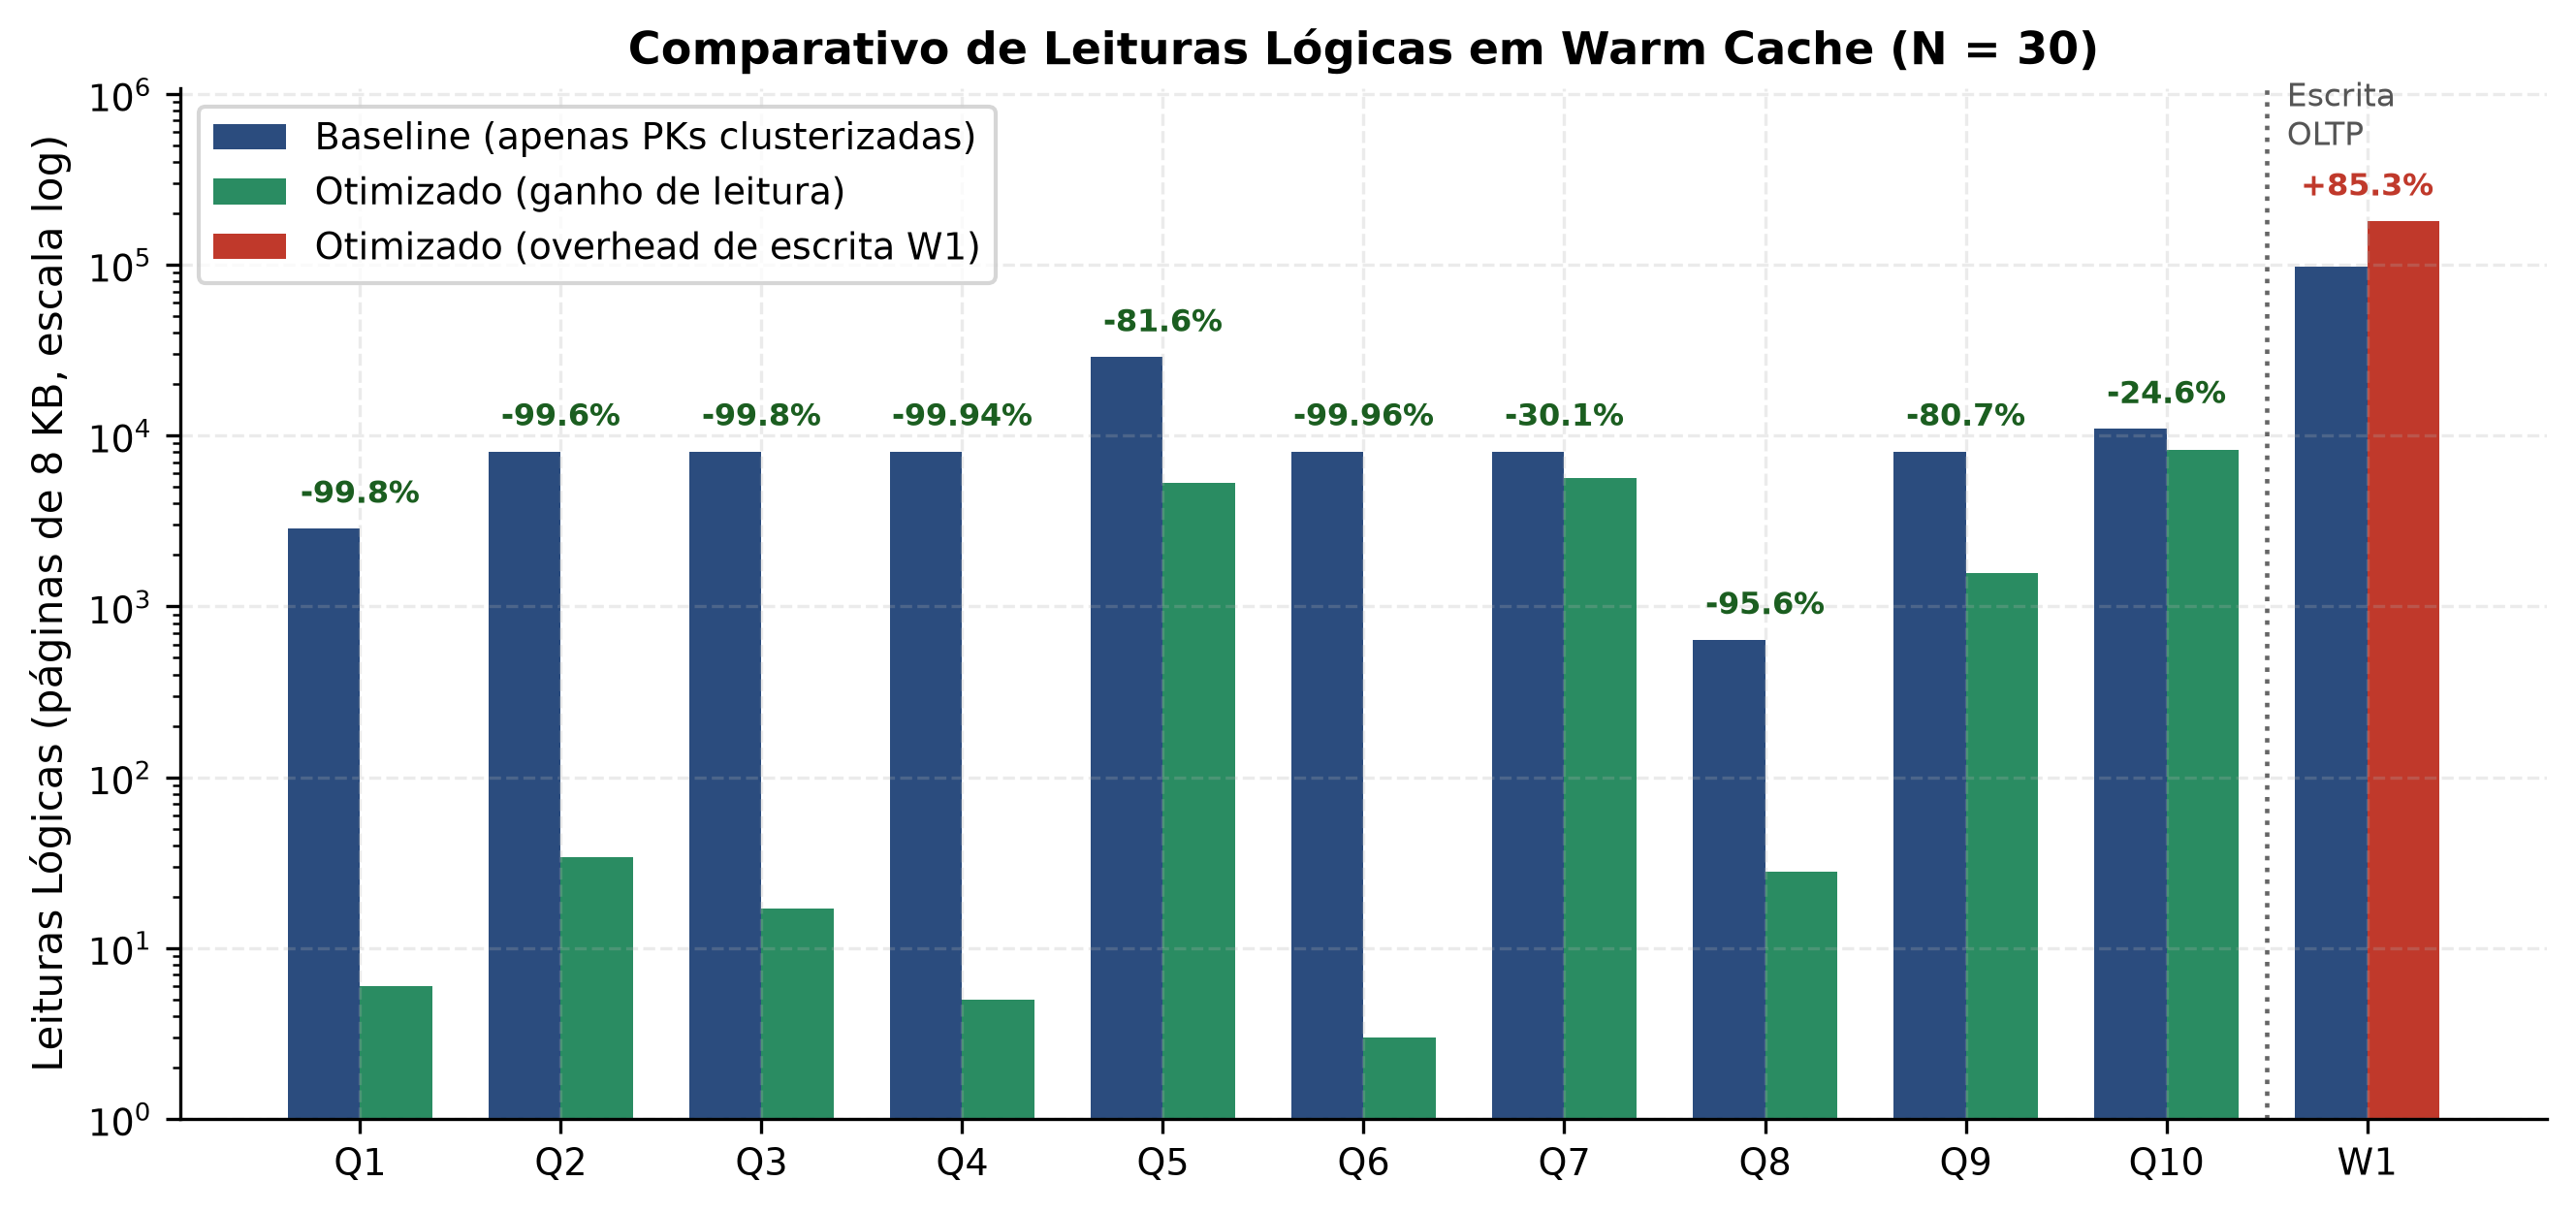
\includegraphics[width=0.73\textwidth]{fig1_leituras_logicas.png}\par
  \vspace{0.3em}
  \footnotesize
  \textbf{Destaques:} reduções de \textbf{99,96\%} ($Q_6$: 8.090 $\rightarrow$ 3), \textbf{99,94\%} ($Q_4$: 8.090 $\rightarrow$ 5), \textbf{99,79\%} ($Q_1, Q_3$) e \textbf{95,60\%} ($Q_8$); escrita $W_1$ elevou E/S em \textbf{+85,33\%} (97.154 $\rightarrow$ 180.057 páginas).
\end{frame}

\begin{frame}{7. Resultados: Latência, Dispersão e \textit{Speedup} ($N=30$)}
  \centering
  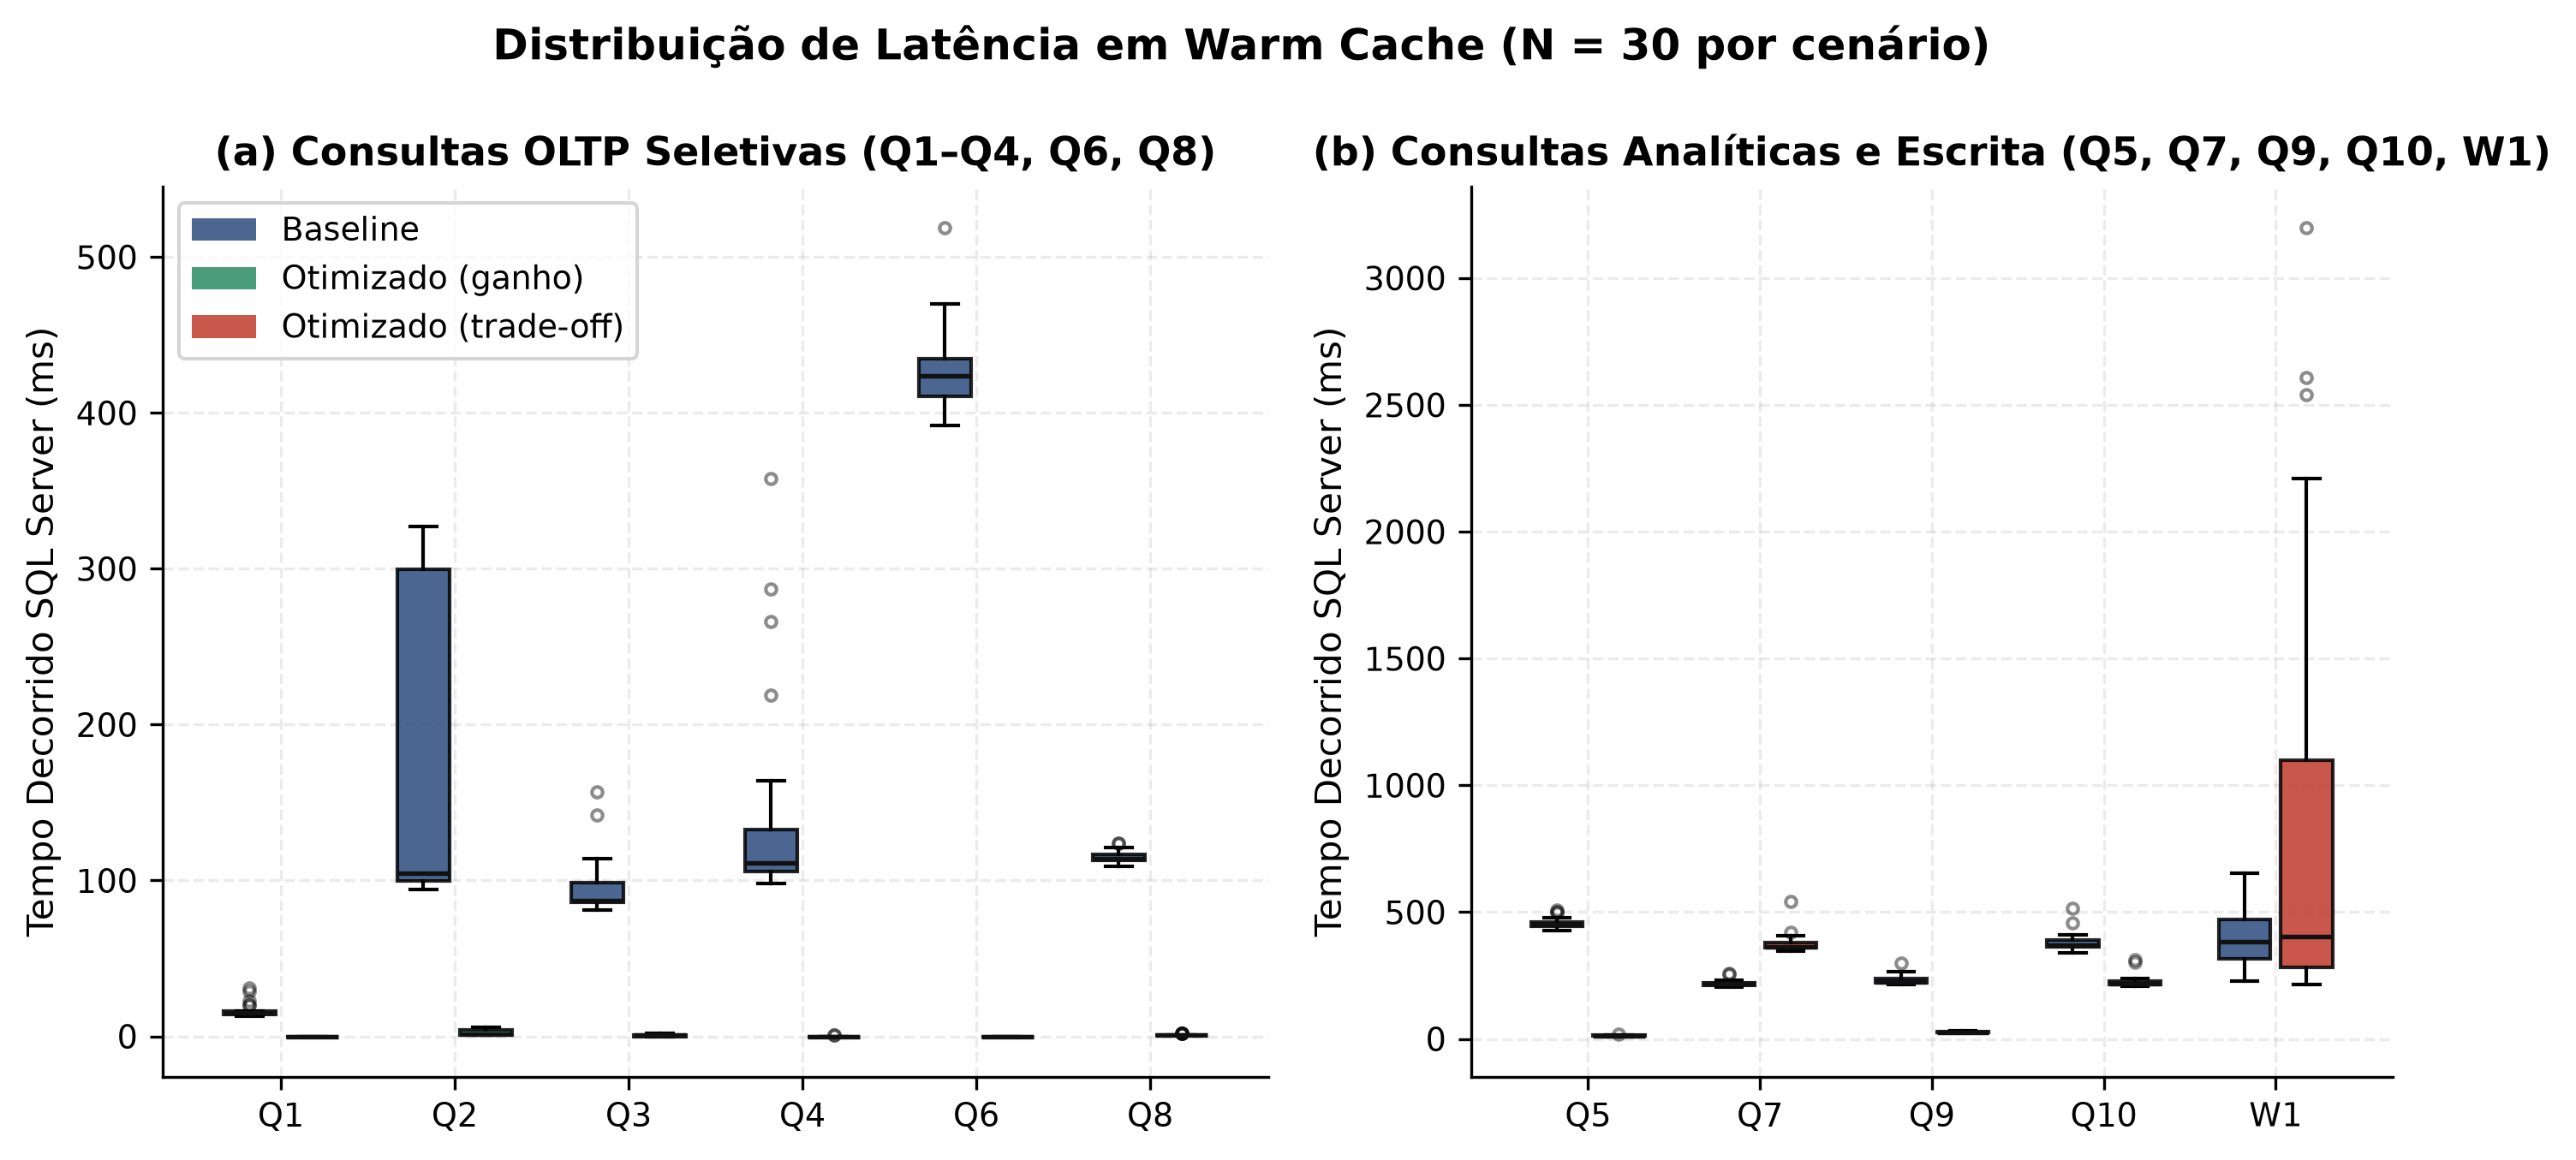
\includegraphics[width=0.82\textwidth]{fig2_tempos_execucao_boxplot.png}\par
  \vspace{0.25em}
  \footnotesize
  \begin{columns}[T]
    \begin{column}{0.48\textwidth}
      \textbf{Maiores acelerações ($p < 10^{-4}$):} $Q_6$ ($>424\times$), $Q_8$ ($114{,}0\times$), $Q_4$ ($>111\times$), $Q_3$ ($87{,}0\times$), $Q_2$ ($69{,}7\times$), $Q_5$ ($37{,}5\times$).
    \end{column}
    \begin{column}{0.48\textwidth}
      \textbf{Trade-offs:} $Q_7$ desacelerou ($0{,}60\times$, $p < 10^{-4}$); $W_1$ teve alta variância em Warm (mediana $404{,}0$ ms; DP $853{,}2$ ms; $p=0{,}129$) e queda em Cold ($0{,}46\times$).
    \end{column}
  \end{columns}
\end{frame}

\begin{frame}{8. Estudo de Caso $Q_4$: Eliminação Progressiva do \textit{Key Lookup}}
  \centering
  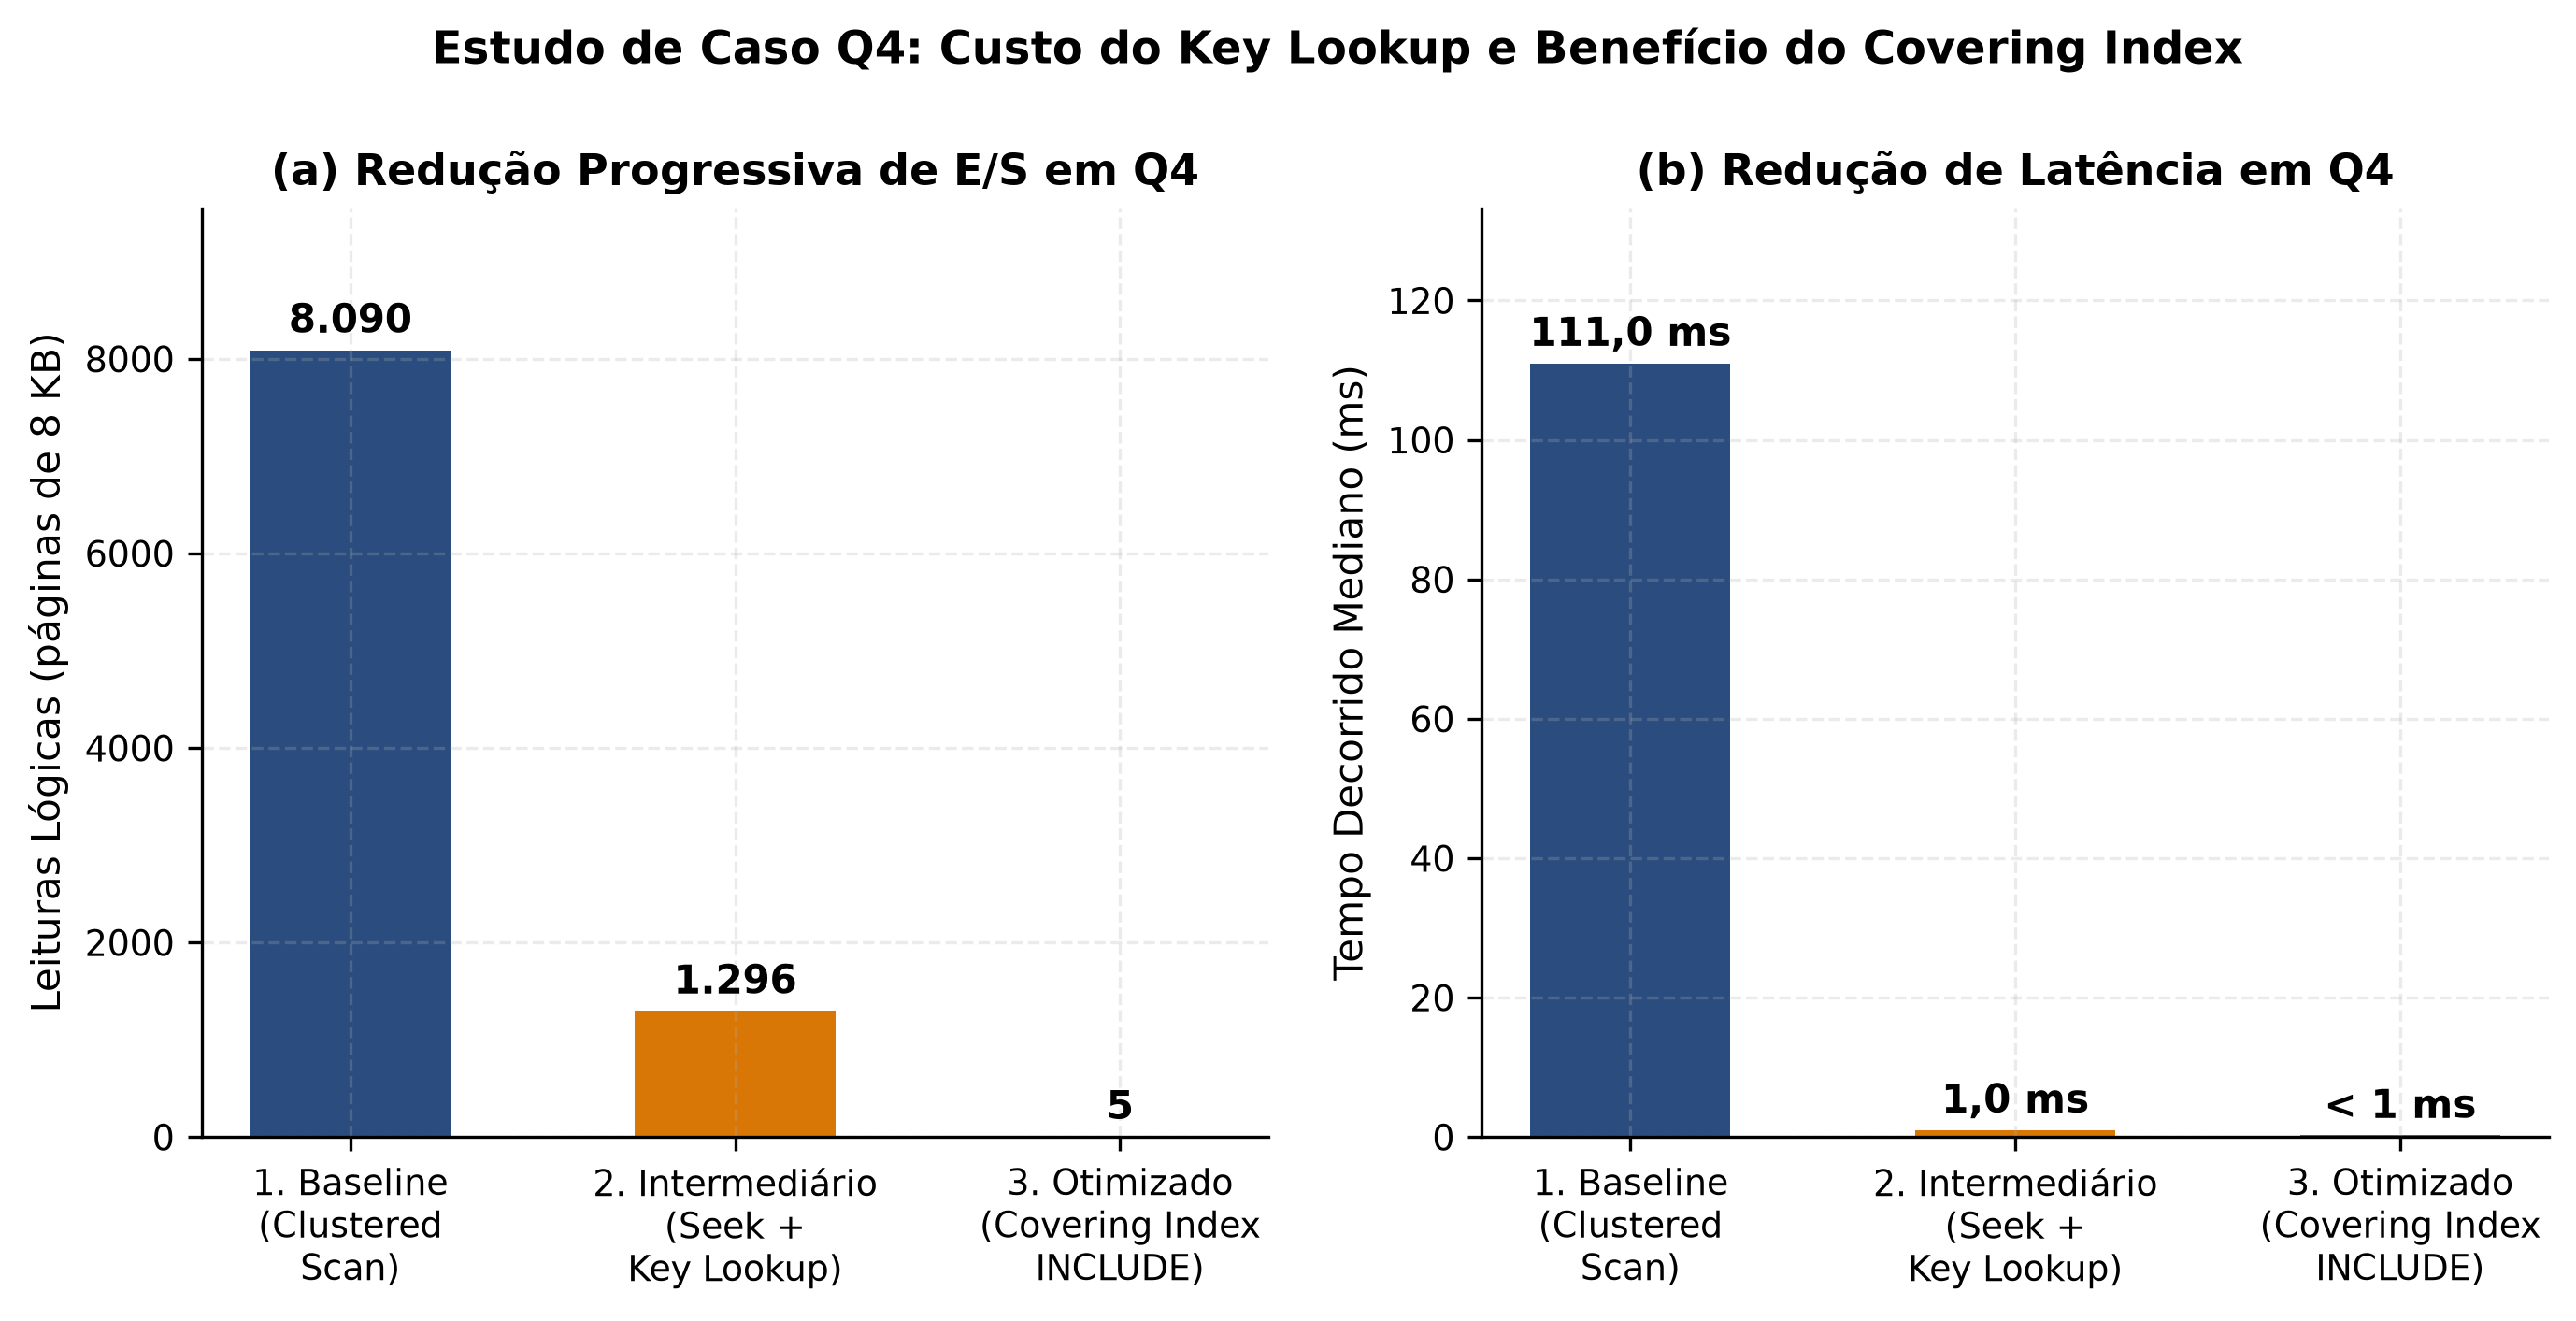
\includegraphics[width=0.75\textwidth]{fig3_q4_tres_estagios.png}\par
  \vspace{0.3em}
  \footnotesize
  \textbf{Progressão:} \textit{Clustered Scan} (\textbf{8.090} pág., 111,0 ms) $\rightarrow$ \textit{Index Seek} + 422 \textit{Key Lookups} (\textbf{1.296} pág.) $\rightarrow$ \textit{Covering Index} com \texttt{INCLUDE} (\textbf{5} pág., $<1$ ms, \textbf{-99,61\%} frente ao estágio intermediário).
\end{frame}

\begin{frame}{9. Anatomia dos Planos Físicos Reais (\texttt{ShowPlanXML})}
  \centering
  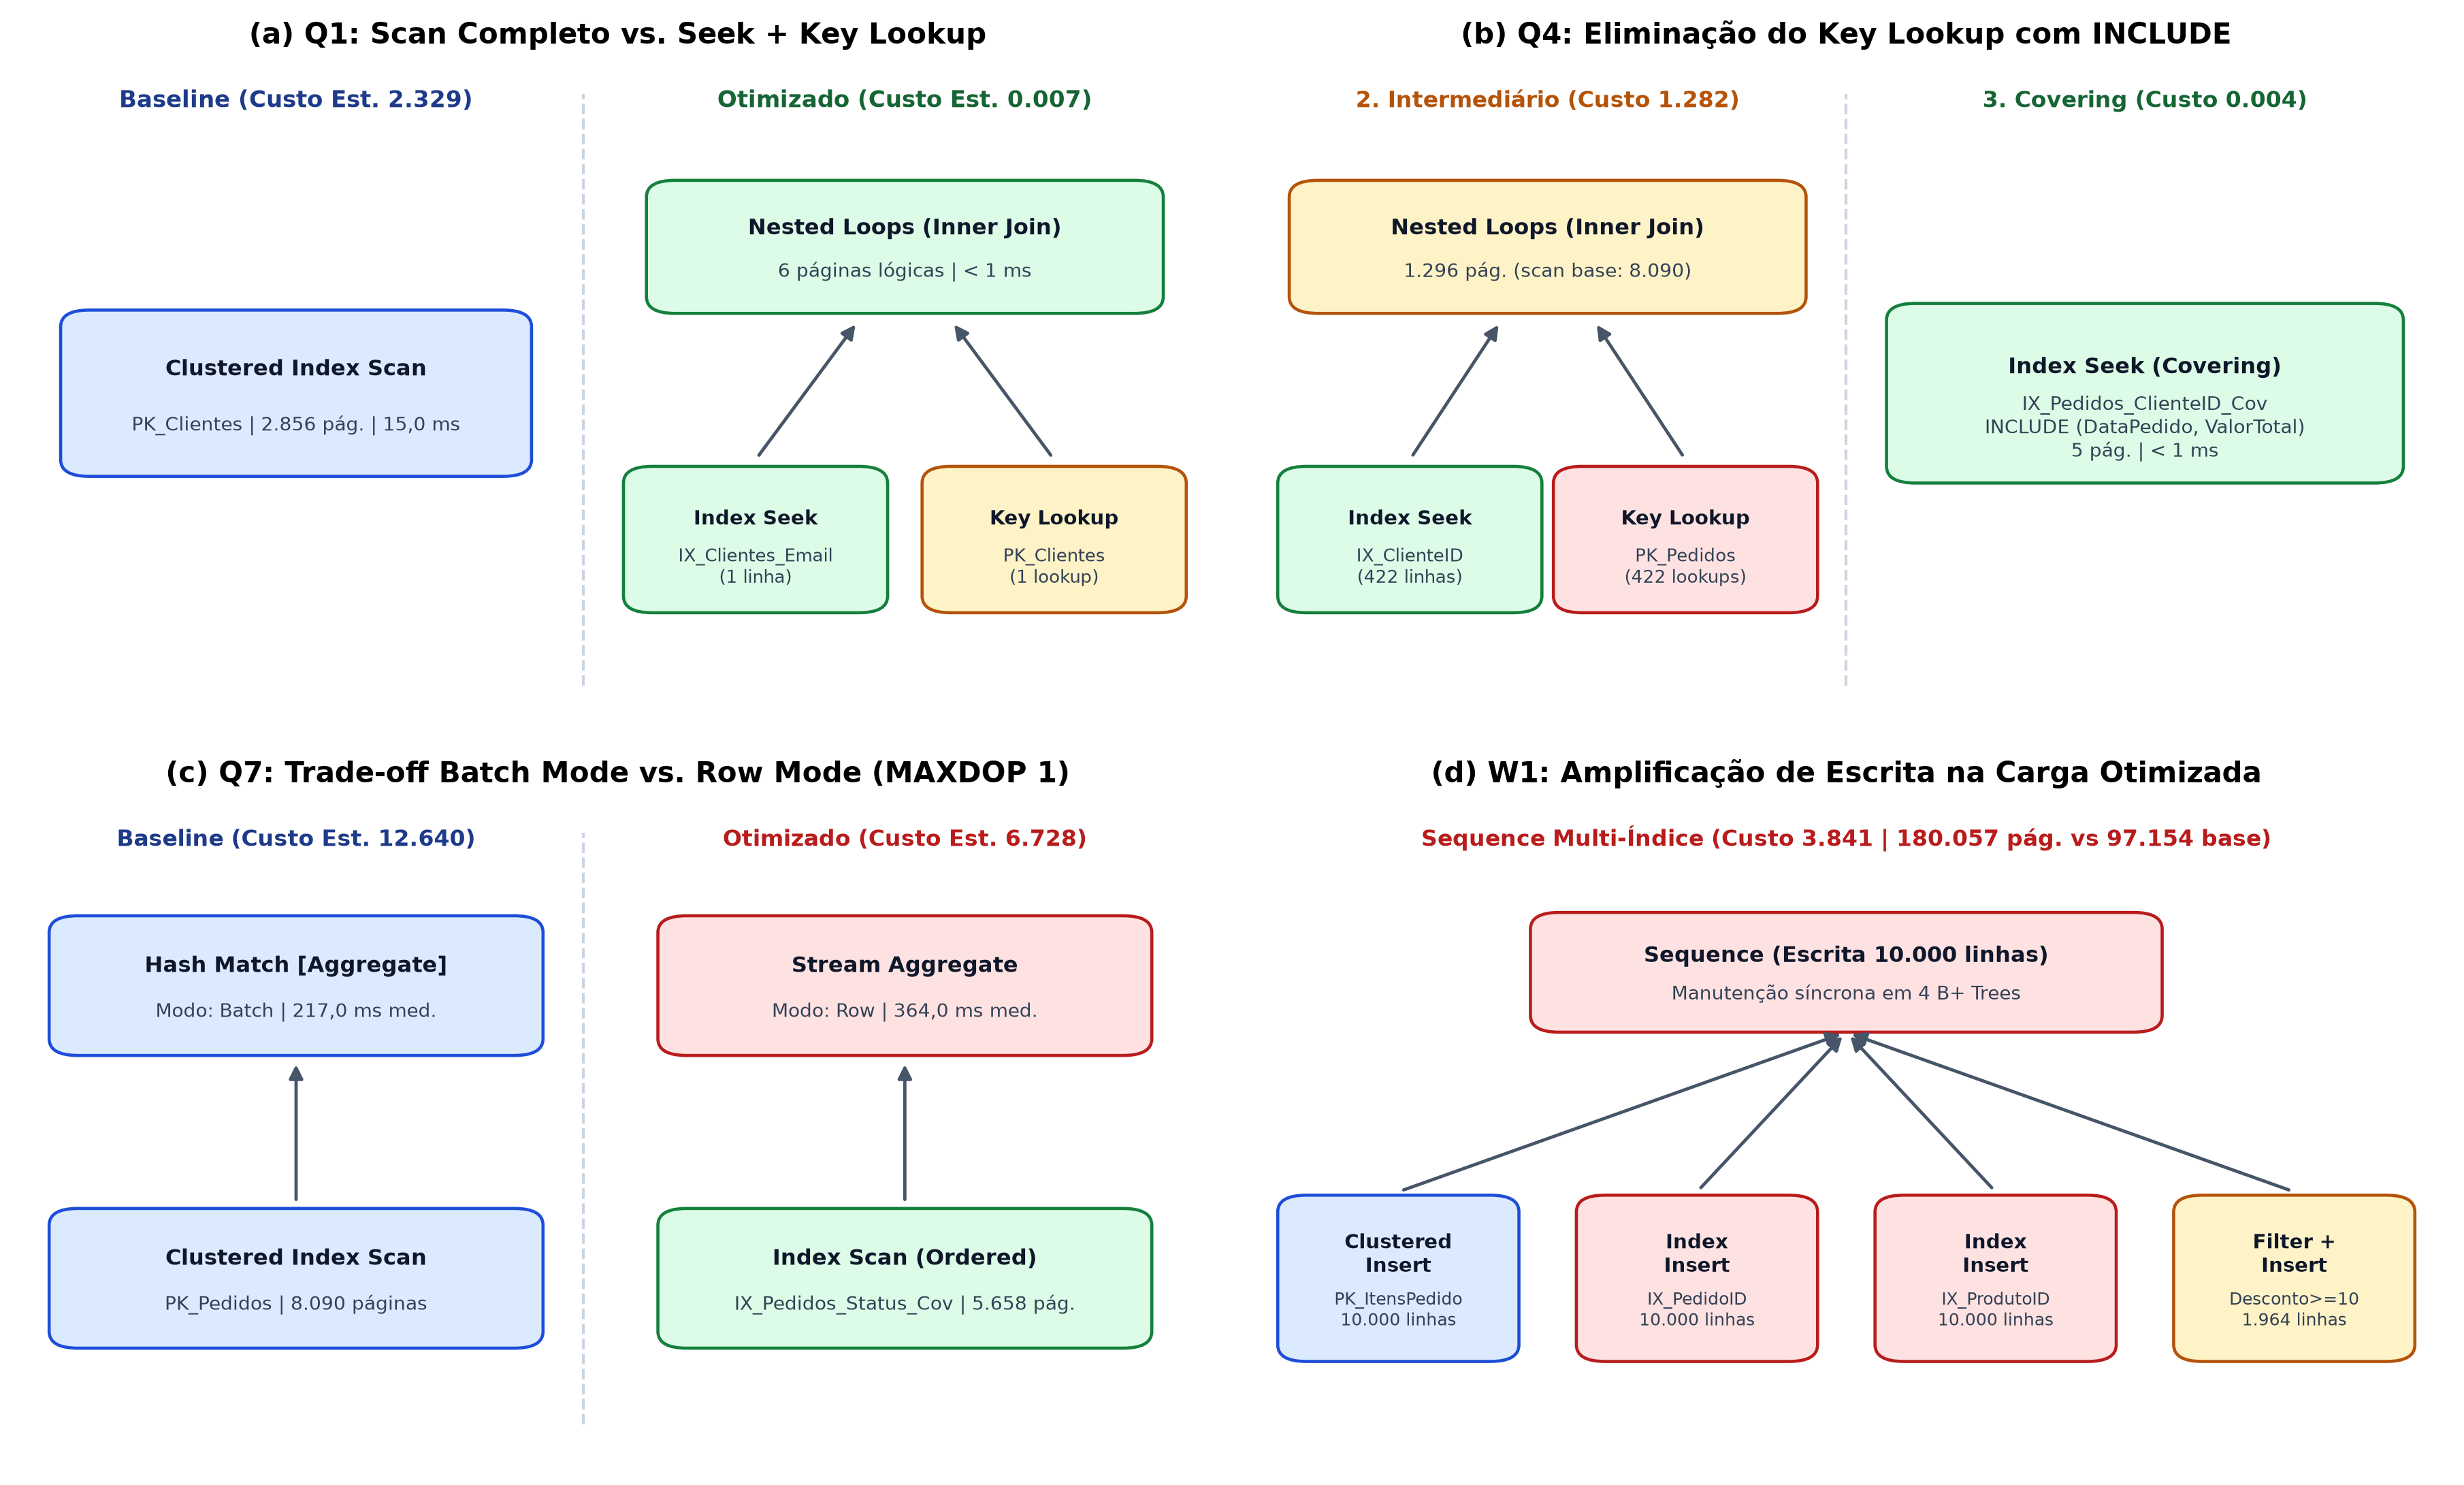
\includegraphics[width=0.73\textwidth]{fig5_planos_execucao.png}
\end{frame}

\begin{frame}{10. Trade-offs Reais: $Q_7$ (\textit{Batch} vs. \textit{Row Mode}), $W_1$ e Cache}
  \begin{columns}[T]
    \begin{column}{0.48\textwidth}
      \begin{alertblock}{Por que $Q_7$ foi mais lenta com menos E/S?}
        \begin{itemize}
          \item Leituras caíram \textbf{30,06\%} (8.090 $\rightarrow$ 5.658 pág.).
          \item \textbf{Baseline (custo est. 12,64):} \textit{Hash Match} executou em \textbf{\textit{Batch Mode on Rowstore}} (217,0 ms).
          \item \textbf{Otimizada (custo est. 6,73):} \textit{Stream Aggregate} operou em \textbf{\textit{Row Mode}} tupla-a-tupla sob \texttt{MAXDOP 1} (364,0 ms; $0{,}60\times$).
        \end{itemize}
      \end{alertblock}
    \end{column}
    \begin{column}{0.48\textwidth}
      \centering
      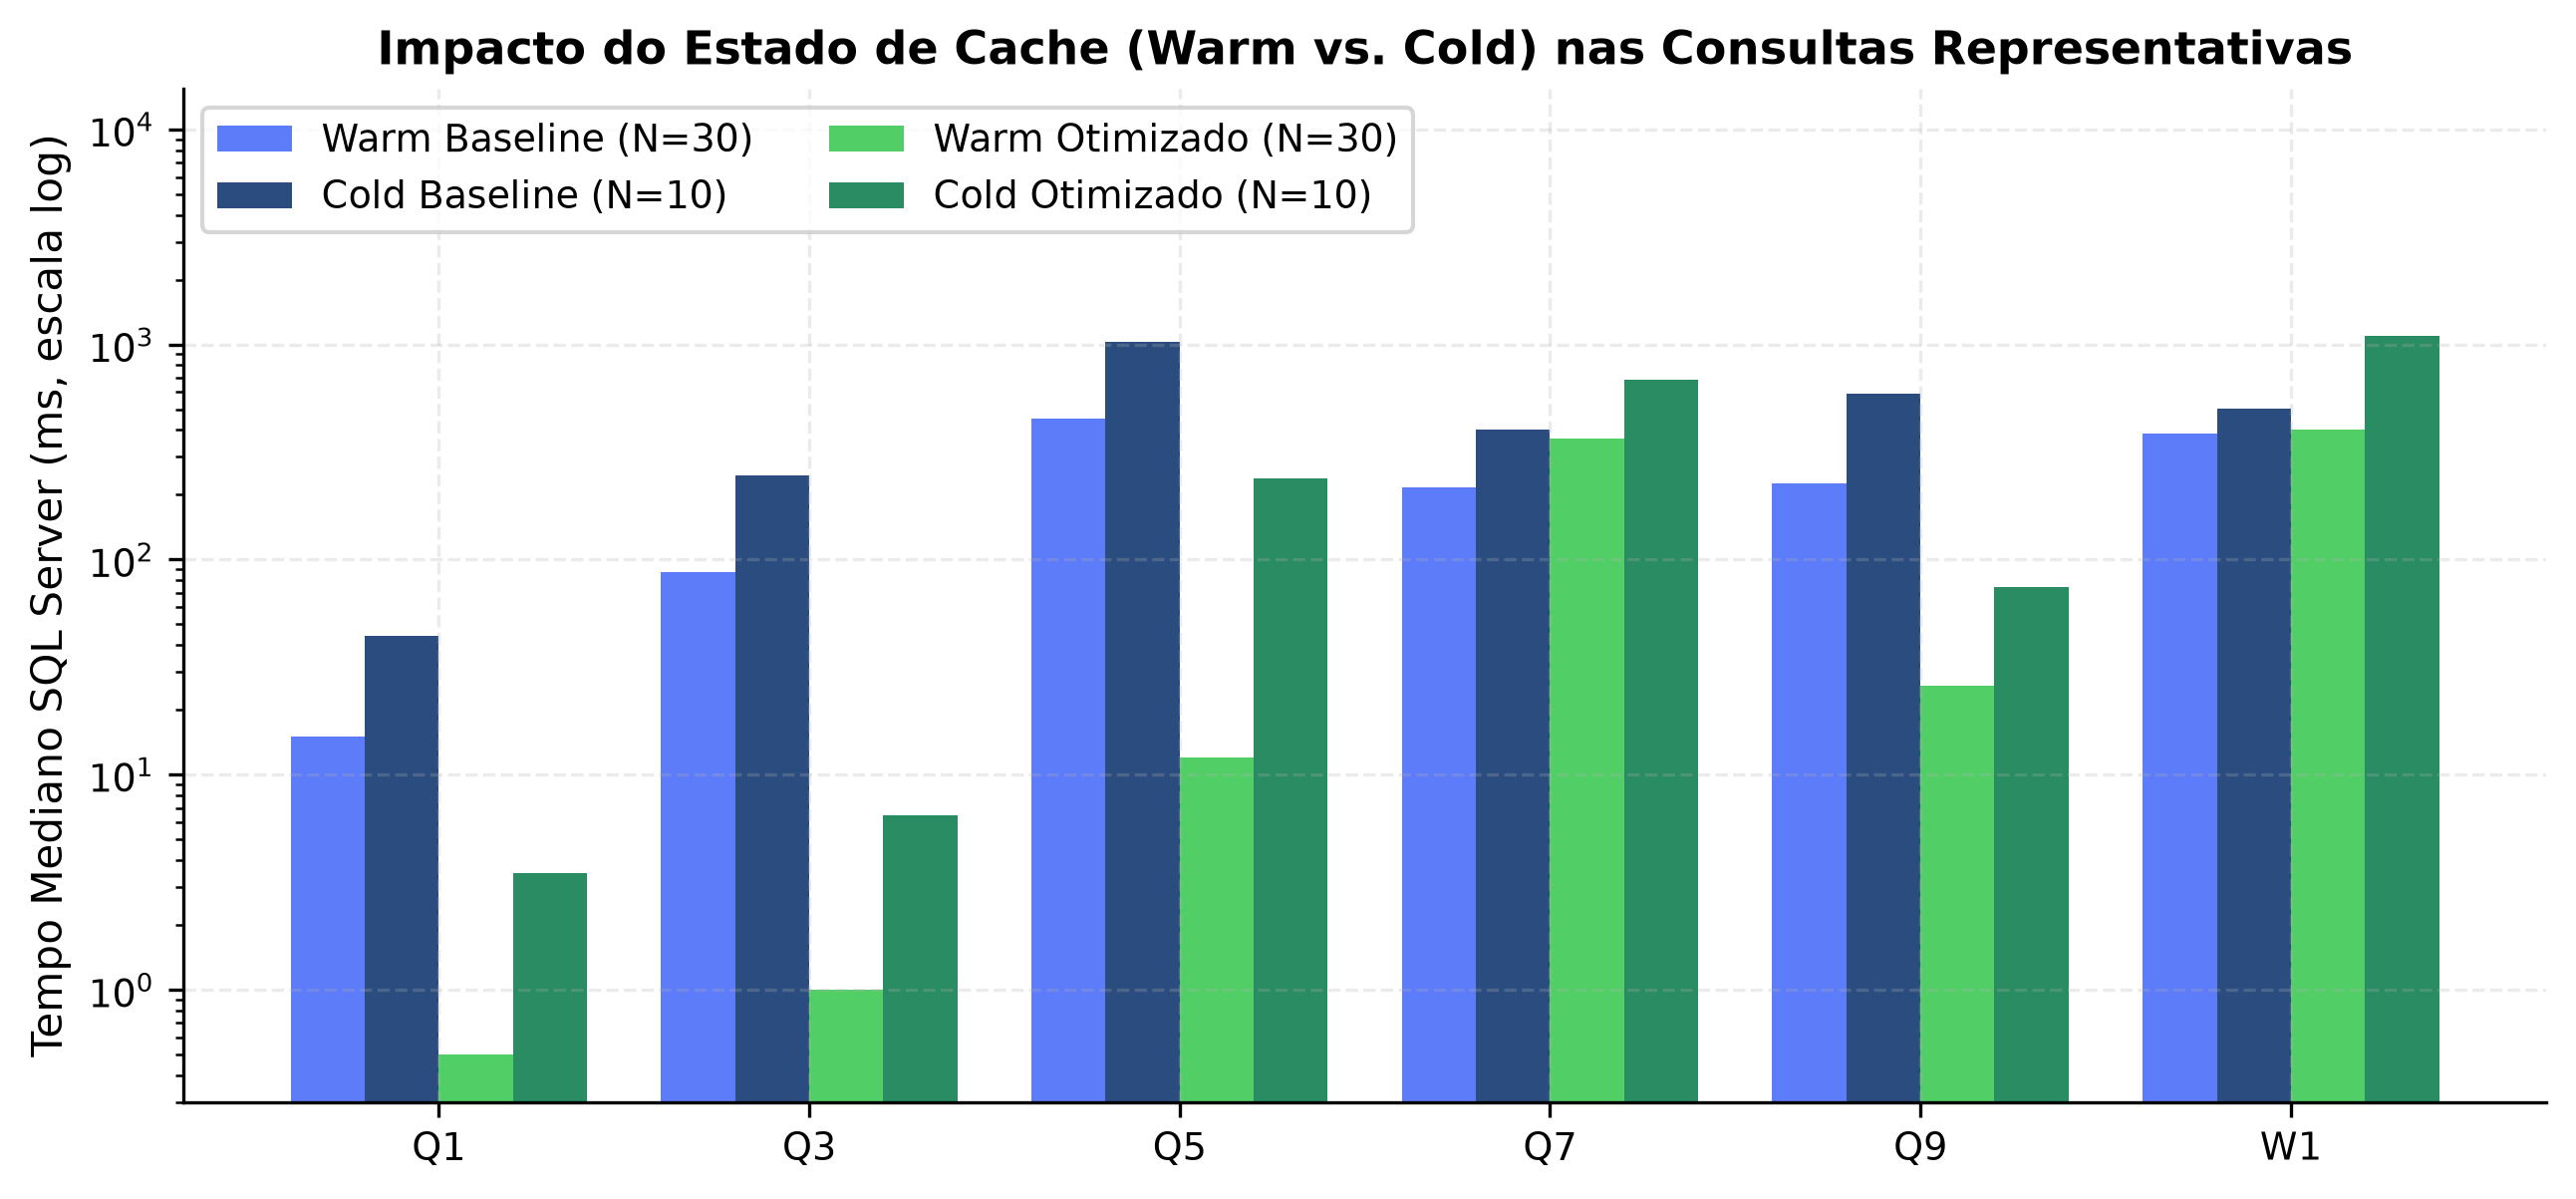
\includegraphics[width=\textwidth]{fig4_warm_vs_cold_cache.png}\par
      \vspace{0.2em}
      \scriptsize
      \textbf{Escrita $W_1$:} \texttt{Sequence} em 4 B+ Trees (incluindo 1.964/10.000 linhas no índice filtrado) elevou leituras em \textbf{+85,33\%} (Warm) e \textbf{+264,73\%} (Cold).
    \end{column}
  \end{columns}
\end{frame}

\begin{frame}{11. Demonstração Prática ao Vivo (4–5 min)}
  \begin{block}{Execução no VS Code (\texttt{mssql}) + \textit{Enable Actual Plan} contra Docker}
    \begin{enumerate}
      \item \textbf{01 -- \texttt{Q1} (Scan vs. Seek):} \texttt{Ecommerce\_Baseline} (\textit{Clustered Index Scan}, 2.856 pág.) vs. \texttt{Ecommerce\_Otimizado} (\textit{Index Seek} + \textit{Lookup}, 6 pág.).
      \item \textbf{02 -- \texttt{Q3} (Índice Composto):} eficiência de \texttt{IX\_Pedidos\_Status\_Data} reduzindo de 8.090 para 17 páginas.
      \item \textbf{03 -- \texttt{Q4} (Eliminação de \textit{Lookup}):} \textit{Index Seek} puro em \texttt{IX\_Pedidos\_ClienteID\_Cov} (5 páginas, sem \textit{Nested Loops}).
      \item \textbf{04 -- \texttt{W1} (Trade-off de Escrita):} \texttt{INSERT} de 10.000 itens sob \texttt{BEGIN TRAN ... ROLLBACK} exibindo os 4 operadores \textit{Insert} (180.057 vs. 97.154 páginas).
    \end{enumerate}
  \end{block}
  \footnotesize \textbf{Contingência:} planos \texttt{.sqlplan} pré-capturados e vídeo de backup prontos em caso de falha de rede/Docker.
\end{frame}

\begin{frame}{12. Conclusões e Lições de Engenharia}
  \begin{columns}[T]
    \begin{column}{0.52\textwidth}
      \begin{exampleblock}{Síntese das Contribuições}
        \begin{itemize}
          \item Reduções de até \textbf{99,96\% em E/S} e aceleração superior a \textbf{424$\times$} em leituras seletivas.
          \item Prova empírica da eliminação de \textit{Key Lookups} via \texttt{INCLUDE} e da recuperação de sargabilidade ($Q_8, Q_9$).
          \item Evidência concreta dos limites: sobrecarga de escrita em $W_1$ e impacto de \textit{Batch Mode} em $Q_7$.
        \end{itemize}
      \end{exampleblock}
    \end{column}
    \begin{column}{0.44\textwidth}
      \begin{block}{Regras Práticas e Trabalhos Futuros}
        \begin{itemize}
          \item Indexar pelo perfil global (leitura vs. escrita), priorizando cobertura e filtros seletivos.
          \item Validar planos reais (\texttt{ShowPlanXML}) e não apenas contagens de páginas.
          \item \textbf{Futuro:} paralelismo multi-thread, índices \textit{Columnstore} para $Q_7$ e cargas mistas concorrentes.
        \end{itemize}
      \end{block}
    \end{column}
  \end{columns}
  \vspace{0.4em}
  \centering
  \textbf{Obrigado! Perguntas e Discussão}
\end{frame}

\end{document}
